\documentclass[../main.tex]{subfiles}
\begin{document}
\onlyinsubfile{
\setcounter{chapter}{8}
}
\notinsubfile{
}
\chapter{eindopdracht: werken in w}
\onlyinsubfile{
%\marginnote{%\vspace{0cm}
%\textcolor{red}{hoofdstuk is los gecompileerd, hstk nummer is \thechapter}
%}
}
\notinsubfile{
%\marginnote{\vspace{0cm}
%\textcolor{red}{main.tex gecompileerd, nummering zou moeten kloppen}}
}


\section{Overgangen op de eenheidscirkel}
\nogdoen{
In figuur 3.2 is te zien wat de x-poort doet met een toestand. Bedacht moet worden dat de eenheidscirkel ook kan worden opgevat als een verzameling punten in het x-y-vlak. Verwisseling van co\"ordinaten komt dan neer op spiegeling om de y=x-lijn. Spiegelingen laten lengtes en hoeken onveranderd. Dus het inwendig product van twee vectoren verandert ook niet. 
Hoe zit dat bij andere poorten?
De volgende poort die we onderzoeken is de \port{Z}-poort. We kijken eerst weer naar wat de poort doet met de basistoestanden, leiden daaruit af wat de poort doet met een willekeurige toestand en daarna kijken we naar de grafische representatie op de eenheidscirkel.
De $\port{Z}$-poort
Het gedrag van een poort is bekend op het moment dat je weet wat de poort doet met de basistoestanden $\ket{0}$ en $\ket{1}$.
Voor de $\port{Z}$-poort geldt:
$\port{Z}\ket{0} = \ket{0}$. Dat betekent dus dat de $\port{Z}$-poort niets doet met de toestand $\ket{0}$. Zou de poort met de toestand $\ket{1}$ ook niets doen dan zou de poort iedere toestand ongewijzigd laten. Zo'n poort heeft in ieder geval theoretisch nut zoals we later zullen zien. De \port{Z}-poort doet echter wel iets met de toestand $\ket{1}$. Er geldt:
$\port{Z}\ket{1} =\ket{-1}$. Voor de algemene werking van de poort betekent dat:
}
\nogdoen{invoegen}

\begin{mdframed}[style=wiskader,frametitle={Matrixen}]
\section{Wiskundekader 4 Productrruimte}
Met objecten uit een twee-dimensionele wereld kan een koppeling tot stand worden gebracht tussen de vier-dimensionele wereld en de twee-dimensionele wereld. Dat kan gebeuren met behulp van vectoren uit twee-dimensionele ruimtes .
We nemen een vector \vect{a} uit de twee-dimensionele ruimte V1 
We nemen een vector \vect{b} uit de twee-dimensionele ruimte V2 
Aan beide vectoren voegen we nu een vector $\vect{a} \otimes \vect{b}$ toe uit de vier-dimensionale ruimte W.
Als we de vier basisvectoren uit W koppelen aan de basisvectoren uit de twee-dimensionele ruimten V1 en V2 zijn we klaar want dan volgt de rest vanzelf.
Hiernaast staat de koppeling aan de basisvectoren uit de vier-dimensionele ruimte W.

\marginnote{%
\[\smqty(1\\0\\0\\0) \equiv \smqty(1\\0)\otimes\smqty(1\\0)\]
\[\smqty(0\\1\\0\\0) \equiv \smqty(1\\0)\otimes\smqty(0\\1)\]
\[\smqty(0\\0\\1\\0) \equiv \smqty(0\\1)\otimes\smqty(1\\0)\]
\[\smqty(0\\0\\0\\1) \equiv \smqty(0\\1)\otimes\smqty(0\\1)\]
}
Bedenk dat dit een keuze is. De eerste basisvector uit de vier-dimensionele ruimte W wordt toegekend aan de beide eerste basisvectoren uit de ruimten V1 en V2.
Andere afspraken waren heel goed mogelijk geweest maar niet verstandig! Met name de verwisseling van de twee binnenste vindt vaak plaats en dan wordt het een rommeltje!
De vierdimensionale vector $\vect{a} \otimes \vect{p}$ kan nu worden gevonden door te bedenken dat deze vector een lineaire combinatie is van de vierdimensionale basisvectoren. 
Stel dat $\vect{a} = \mqty(a\\b)$ en dat $\vect{p} = \mqty(p\\q)$ 
Omdat $\vect{a}\otimes \vect{p}$ deel uitmaakt van de vier-dimensionele ruimte geldt het volgende:

\[\mqty(\alpha\\ \beta\\ \gamma\\ \delta)=\alpha\mqty(1\\0\\0\\0) + \beta\mqty(0\\0\\0\\1) +\gamma\mqty(0\\0\\1\\0) +\delta\mqty(0\\0\\0\\1) \]

Maar ook geldt:
\begin{align*}
\vect{a} \otimes \vect{p} & =\mqty(a\\b) \otimes \mqty(p\\q)\\
& =\left[a\mqty(1\\0) + b\mqty(1\\0)\right] \otimes \left[p\mqty(1\\0) + q\mqty(1\\0)\right]\\
& = ap\mqty(1\\0) \otimes \mqty(1\\0) + 
    aq\mqty(1\\0) \otimes \mqty(0\\1) + 
    bp\mqty(0\\1) \otimes \mqty(1\\0) + 
    bq\mqty(1\\1) \otimes \mqty(1\\1)\\
& = ap\mqty(1\\0\\0\\0) + 
    aq\mqty(1\\0\\0\\0) + 
    bp\mqty(1\\0\\0\\0) + 
    bq\mqty(1\\0\\0\\0) = \mqty(ap\\aq\\bp\\bq)
\end{align*}

Snel even een oefening. \nogdoen{Opgave 3.12}.

\begin{antwoord}
niet genormeerde vectoren
\begin{enumerate}
  \item $\smqty(1\\0\\0\\0)$
  \item $\smqty(1\\0\\0\\0)$
\end{enumerate}
\end{antwoord}
\begin{opdracht}
\begin{enumerate}
\item Bereken $\mqty(\tfrac{1}{2} \\ \tfrac{1}{2}\sqrt{3}) \otimes \mqty(\tfrac{1}{\sqrt{5}} \\ \tfrac{2}{\sqrt{5}})$
\item Bereken $\mqty(0\\1) \otimes \mqty(\tfrac{1}{\sqrt{5}} \\ \tfrac{2}{\sqrt{5}})$
\end{enumerate}
\end{opdracht}

De weg terug van W naar de afzonderlijke ruimten V1 en V2 is wat lastiger. \nogdoen{Opgave 3.13}.

\begin{antwoord}
niet genormeerde vectoren
\begin{enumerate}
  \item $...$
  \item $...$
\end{enumerate}
\end{antwoord}
\begin{opdracht}
Voor een product geldt $\vect{a} \otimes \vect{p} =\mqty(a\\b) \otimes \mqty(p\\q)==\mqty(2\\3) \otimes \mqty(4\\6)$
\begin{enumerate}
\item Bereken de waarden van de co\"efficienten a, b, p en q. 
\item Normaliseer de vierdimensionale vector en vindt opnieuw de constanten a,b,p en q. 
\end{enumerate}
\end{opdracht}

Er doet zich een merkwaardig probleem voor.

\nogdoen{Opgave 3.14} brengt dat aan het licht. 

\begin{antwoord}
(tensorproduct)
\begin{enumerate}
  \item $...$
  \item $...$
  \item $...$
  \item $...$
\end{enumerate}
\end{antwoord}
\begin{opdracht}
Er bestaat geen enkel product $\vect{a} \otimes \vect{p} =\mqty(a\\b) \otimes \mqty(p\\q)= \mqty(2\\3\\0\\6)$. 
\begin{enumerate}
\item Leg uit waarom niet. 
\item Waarom moet er zeker nog een andere component nul zijn?
\item Verander de getoonde 4-vector zodanig dat er wel een oplossing is.
\item Is er nog een alternatief?
\end{enumerate}
\end{opdracht}
 
\nogdoen{Opgave 2.16} toont aan dat er vectoren zijn in de vier-dimensionale ruimte W die niet gekoppeld zijn aan vectoren uit de twee-dimensionale ruimte. De productruimte $V_1 \otimes V_2$ blijkt maar een kleine deelverzameling van de vierdimensionale ruimte $W$ te zijn.
Kijken we nog eens naar alle mogelijke vectoren uit de productruimte $V_1 \otimes V_2$.
Neem een willekeurige vector $\vect{a} = \mqty(a\\b)$ uit $V_1$ en een willekeurige vector$\vect{p} = \mqty(p\\q)$ uit $V_2$ In dat geval moet voor een vector uit de productruimte$V_1 \otimes V_2$ altijd gelden dat de componenten gelijk zijn aan 


\[ \mqty(ap\\aq\\bp\\bq)\]

De binnenste twee componenten vermenigvuldigen levert op $aqbp$. 
De buitenste twee componenten vermenigvuldigen levert op $apbq$

Voor vectoren uit de productruimte moet blijkbaar gelden dat het product van de binnenste twee componenten gelijk is aan de buitenste twee componenten. Voor vectoren uit de vierdimensionale ruimte W geldt die forse beperking niet. Vectoren uit die ruimte , bijvoorbeeld, met maar \'e\'en component gelijk aan nul, kunnen nooit in de productruimte zitten. De vier basisvectoren zitten wel in de productruimte want dat is het gevolg van de definitie geweest. Drie componenten gelijk aan nul is dus geen probleem.

\begin{antwoord}
2comp=0
\end{antwoord}
\begin{opdracht}
Hoe zit het met twee componenten gelijk aan nul?
\end{opdracht}
 
Figuur~\ref{fig:stoffigeruimte2} brengt een en ander nog eens in beeld.
 
\begin{center}
\leavevmode
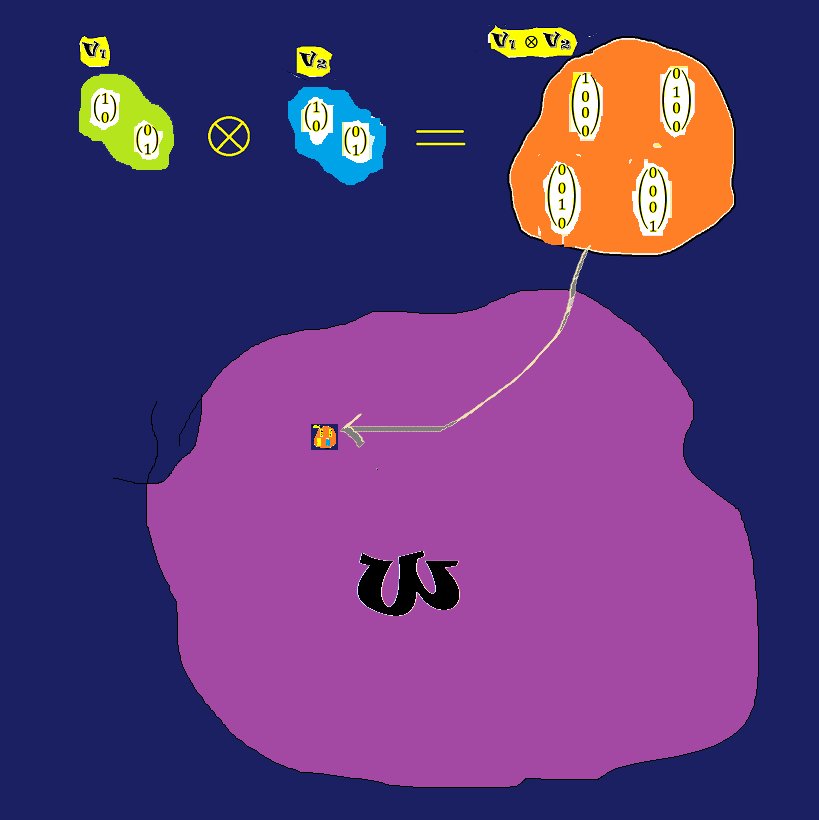
\includegraphics[width=0.5\textwidth]{./img/prodruimtev1v2.png}
 \captionof{figure}{De productruimte $V_1 \otimes V_2 $ maakt deel uit van de veel grotere vier-dimensionale ruimte $W$. De basisvectoren waarmee de hele vierdimensionale ruimte kan worden opgespannen zitten wel in de productruimte. 
\label {fig:stoffigeruimte2}}
\end{center}

\section{Producten van matrices}
In de vier-dimensionele ruimte $W$ kan ook gewerkt worden met matrices die vectoren afbeelden op andere vectoren. 
Ook bij matrices \matr{A} en \matr{B} bestaat er een productmatrix $\matr{A}\otimes \matr{B}$. 

Stel  $\matr{A} = \mqty(a & b \\ c&d)$en $\matr{B} = \mqty(q&r \\ s & t)$
 
$\matr{A} \otimes \matr{A} = \mqty(a\matr{B} & b\matr{B} \\ c\matr{B}&d\matr{B}) = \mqty(a\mqty(q&r \\ s & t) & b\mqty(q&r \\ s & t) \\ c\mqty(q&r \\ s & t) & d\mqty(q&r \\ s & t)) = \mqty(aq &ar & bq &br \\as &at & bs &bt \\ cq &cr &dq &dr\\cs&ct&ds&dt)$

\begin{antwoord}
\begin{enumerate}
\item $...$
\item $...$
\item $...$
\item $...$
\item $...$
\item $...$
\item $...$
\end{enumerate}
\end{antwoord}
\begin{opdracht}
Bekijk de volgende 2x2 matrixen: $I=\mqty{1&0\\0&1}$ en $X=\mqty{0&1\\1&0}$
\begin{enumerate}
\item Bereken $I \otimes X$ en $X \otimes I$
\item Is deze matrixvermenigvuldiging commutatief?
\end{enumerate}
Bekijk de volgende 4x4-matrix $m = \mqty(1 &1 & 0 &0 \\1 &-1 & 0 &0 \\0  &0 &1  &1 \\0 &0 &1 &-1)$
\begin{enumerate}
\item Van welk tensorproduct kan deze matrix afkomstig zijn?
\item Bereken $m=\mqty(1&1) \otimes \mqty(2&0)$
\item Ga na of de berekende vector in de productruimte ligt.
\item Bereken $m=\mqty(a&b) \otimes \mqty(p&q)$
\item Ga na of deze vector altijd in de productruimte ligt.
\end{enumerate}
\end{opdracht}

Als er voor \'e\'en qubit een bewerking \matr{m} bestaat dan bestaat er ook een bewerking \matr{M_2} die hetzelfde doet met de beide qubits van een \nogdoen{biqubit}. Er geldt


\[M_2=M \otimes M\]


\begin{antwoord}
\begin{enumerate}
\item $\matr{X_2}=$, $\matr{X_2}\ket{01}=$.
\item $\matr{Z_2}=$, $\matr{Z_2}\ket{00}=$.
\item $\matr{H_2}=$, $\matr{H_2}\ket{11}=$.
\end{enumerate}
\end{antwoord}
\begin{opdracht}
\begin{enumerate}
\item Stel de matrix van$\matr{X_2}$ op en bereken $\matr{X_2}\ket{01}$.
\item Stel de matrix van$\matr{Z_2}$ op en bereken $\matr{Z_2}\ket{00}$.
\item Stel de matrix van$\matr{H_2}$ op en bereken $\matr{H_2}\ket{11}$.
\end{enumerate}
\end{opdracht}
Algemene stelling

Stel je wilt twee qubits in de toestanden $\ket{x}$ en $\ket{y}$ transformeren met respectievelijk $\matr{A} en \matr{B}$. Daarna zou je het product $\matr{A}\ket{\vect{x}} \otimes \matr{A}\ket{\vect{x}}$ kunnen berekenen. Maar je zou ook de volgorde kunnen omdraaien. Eerst bereken je het product $\ket{\vect{x}} \otimes \ket{\vect{x}}$, vervolgens bereken je de productmatrix $\matr{A} \otimes \matr{B}$. Tenslotte voer je de transformatie uit. Het blijkt voor het antwoord niet uit te maken. Dus:

\[\matr{A}\ket{\vect{x}} \otimes \matr{b}\ket{\vect{y}} = (matr{A} \otimes \matr{B})(\ket{\vect{x}} \otimes \ket{\vect{x}})\]


\begin{antwoord}
2comp=0
\begin{enumerate}
\item ...
\item ...
\item ...
\item ...
\item ...
\item ...
\end{enumerate}
\end{antwoord}
\begin{opdracht}
Om de algemene stelling te testen proberen we hem uit op de transformatie van twee basisvectoren $\ket{1}$ en $\ket{1}$. De transformaties zijn respectievelijk $\matr{X}$ en $\matr{Z}$.
\begin{enumerate}
\item Bereken $\matr{X}\ket{1}$ en $\matr{Z}\ket{0}$
\item Bereken $\matr{X}\ket{1} \otimes \matr{Z}\ket{0}$
\item Bereken $\ket{1} \otimes \ket{0}$
\item Bereken $\matr{X} \otimes \matr{Z}$
\item Bereken $\left(\matr{X} \otimes \matr{Z}\right)\left(\ket{1} \otimes \ket{0} \right)$
\item Bereken En?...Klopt de stelling in dit bijzondere geval?
\end{enumerate}
\end{opdracht}

Einde van dit wiskundekader
\end{mdframed}


\section{Terug naar de qubits, Verstrengeling}
Met de kennis van de eigenschappen van productruimtes is het niet moeilijk meer om te verklaren waarom het niet mogelijk was om de twee qubits te identificeren die het resultaat waren van de volgende schakeling. 

de uitkomst van de bewerking 
\[ \port{CNOT}\left(\alpha\ket{0}+\beta\ket{1},\ket{1}\right) 
 = \port{CNOT}\left(\alpha\ket{01}+\beta\ket{11}\right)%
 = \mqty(0\\ \alpha \\ \beta \\0)\]

Als $\alpha$ en $\beta$ beide ongelijk aan nul zijn valt deze 4vector buiten de productruimte.
Er zijn dus geen twee individuele qubits te vinden om dit probleem op te lossen. 
Toestanden van een biqubit met een vector die buiten de productruimte valt noemen we verstrengeld. 
Maar dan wordt het wel heel lastig om aan schakelingen te rekenen zoals we dat tot nu toe hebben gedaan. Werp maar even een blik op figuur \nogdoen{2.23} om te zien dat dat heel lastig wordt als je niet goed weet wat er langs de lijnen loopt. Maar met het wiskundig instrument van wiskundekader~4 wordt het allemaal veel eenvoudiger. 

\section{De dubbelqubit}
Een belangrijke uitbreiding van het voorgaande is nu dat we het tweekwantenregister of misschien zouden we kunnen zeggen: de biqubit, nu beschouwen als \'e\'en ding dat vier onbetwijfelbaar verschillende toestanden kent, nl $\ket{00}$ , $\ket{01}$, $\ket{10}$ en $\ket{11}$. Er bestaat dus een meetapparaat A waarmee ondubbelzinnig kan worden vastgesteld in welke van de vier toestanden de biqubit zich bevindt.
De biqubit kan ook in een toestand van superpositie verkeren. We zullen die toestand voor het gemak ook maar weer $\ket{\Psi}$ noemen.
Voor die toestand geldt dan: $\ket{\Psi} =\alpha\ket{00} + \beta\ket{01} + \gamma\ket{10} +\delta\ket{11}$.
Wordt er een meting verricht met apparaat A dan komt daar weer een van de vier basistoestanden uit. Om de toestand $\ket{\Psi}$ te identificeren zijn er weer vele metingen nodig zodat er statistiek kan worden bedreven. De co\"effici\"enten $\alpha$, $\beta$, $\gamma$ en $\delta$ zijn weer amplitudes waarvoor geldt  dat het kwadraat de kans aangeeft om de biqubit aan te treffen in de bijbehorende basistoestand.		
\[\alpha^2 + \beta^2+ +\gamma^2+\delta^2 = 1\]
Net als bij de enkelvoudige qubit kan aan een biqubit ook weer een vector worden toegewezen. Tot nu toe hebben we steeds verschillende symbolen gebruikt om goed duidelijk te maken dat een toestand niet hetzelfde is als een vector. Maar dat wordt nu toch lastig omdat we dan veel te veel symbolen krijgen. Dus afspraak:
$\ket{0}$ en $\ket{1}$ zijn voortaan niet alleen toestanden maar ook symbolen voor de bijbehorende vectoren. Verwarring kan nooit ontstaan want de toewijzing van vectoren aan toestanden is uniek. 
Voor het gemak maken we het voorgaande nog even zichtbaar in figuur \nogdoen{3.13}

\begin{antwoord}
\end{antwoord}
\begin{opdracht}
Neem aan dat twee qubits in de volgende toestanden verkeren:
$\ket{\phi}$ = $\frac{1}{2}\sqrt{3}\ket{0} + \frac{1}{2}\ket{1}$ en $\ket{\Psi}$ = $\frac{1}{2}\sqrt{2}\ket{0} + \frac{1}{2}\sqrt{2} \ket{1}$
Voor de biqubit geldt dan $\ket{\Psi} \alpha \ket{00} + \beta\ket{01} + \gamma\ket{10} + \delta\ket{11}$.
\begin{enumerate}
\item Bereken het product $\ket{\Psi}$ = $\ket{\phi} \otimes \ket{\Psi}$ volgens het schema van \nogdoen{figuur 5.3}
\item Bereken de co\"effici\"enten $\alpha$, $\beta$, $\gamma$ en $\delta$ en ga na dat $\alpha^2 + \beta^2 + \gamma^2 + \delta^2 = 1$
\end{enumerate}
\end{opdracht}

\section{Operatoren in de productruimte}
Nu duidelijk is hoe vectoren in de productruimte er uit zien ligt de stap naar de operatoren voor de hand. Vraag is dan natuurlijk hoe de matrix van de \port{CNOT}-poort er uitziet. Probleem is hier dat van alle denkbare 4x4-matrices slechts een klein deel gevormd wordt door tensorproducten van 2x2 matrices. En ook de \port{CNOT}-matrix is niet zo'n product. 
Maar dit vormt geen probleem 
We weten wat de poort doet met de vier basistoestanden. De matrix bestaat dan uit kolommen van de beeldvectoren van de geordende basisvectoren. In figuur \nogdoen{3.14} is het resultaat te vinden.


Met de poorten \port{CNOT}, \port{X}, \port{Z} en \port{H} kunnen al heel wat poorten worden bestudeerd.

In \nogdoen{figuur 3.15} staan vier schakelingen getekend. 


\begin{antwoord}
\end{antwoord}
\begin{opdracht}
\begin{enumerate}
\item Bepaal de uitkomst van schakeling 1.
\item Bepaal de uitkomst van schakeling 2. 
\item Bepaal de uitkomst van schakeling 3.
\end{enumerate}
\end{opdracht}

\section{Werken in W}
Als een superpositie wordt aangeboden aan de controlingang van een \port{CNOT}-poort ontstaat een verstrengeld qubitpaar. Het is dan niet meer mogelijk om te bepalen wat de invoer is van een individuele poort op een van de lijnen. 
Als voorbeeld de schakeling in figuur 3.16.

Het is onmogelijk om aan te geven welke bit er wordt aangeboden aan de tweede Hadamardpoort. Na de \port{CNOT}-poort is een verstrengelde biqubit ontstaan. Hoe moet dit soort situaties worden onderzocht?
Het antwoord ligt verscholen in de algemene stelling van wiskundekader 4. Overschakelen op werken in de vier-dimensionale ruimte W. Allereerst brengen we een kosmetische verandering aan door de schakeling iets anders te tekenen.


De eenheidspoorten doen niets met de qubits. Maar nu is het wel mogelijk om het probleem anders te zien. De beide individuele bits vervangen we door het tensorproduct. Hetzelfde doen we met de matrices. De algemene stelling zegt dat dat de uitkomst niet zal veranderen.
Dan ontstaat het volgende plaatje: figuur 2.25.

De situatie is nu veel eenvoudiger geworden. We hebben gebruik gemaakt van de algemene stelling uit het wiskundekader~4. 

Eerst maar de biqubit: 


\[ (\alpha\ket{0}+\beta\ket{1}) \otimes \ket{1}\ = \alpha\ket{01}+\beta\ket{11}\]

Dus dan weten we 

\[ input=\mqty(0\\ \alpha\\0\\ \beta)\]

Voor de poorten geldt dat de \port{CNOT}-matrix bekend is en dat de matrix van $\port{I} \otimes\port{H}$ berekend kan worden. Er geldt:

\[ 
\mqty(1&0\\0&1)\otimes\frac{1}{\sqrt{2}}\mqty(1&1\\1&-1)
\mqty(1H&0H\\0H&1H)=\frac{1}{\sqrt{2}}
\mqty(1&1&0&0\\1&-1&0&0\\0&0&1&1\\0&0&1&-1)
\]

Drie bewerkingen vervolgens toepassen op de input geeft het volgende:

\[
(?)=\frac{1}{2}
\mqty(1&1&0&0\\1&-1&0&0\\0&0&1&1\\0&0&1&-1)
\mqty(1&0&0&0\\0&1&0&0\\0&0&1&0\\0&0&0&1)
\mqty(1&1&0&0\\0&-1&0&0\\0&0&1&1\\0&0&1&-1)
\mqty(0\\ \alpha\\0\\ \beta)=
\]


\[
\frac{1}{2}
\mqty(1&1&0&0\\1&-1&0&0\\0&0&1&1\\0&0&1&-1)
\mqty(1&0&0&0\\0&1&0&0\\0&0&1&0\\0&0&0&1)
\mqty(\alpha\\-\alpha\\ \beta\\-\beta)=
\]

\[
\frac{1}{2}
\mqty(1&1&0&0\\1&-1&0&0\\0&0&1&1\\0&0&1&-1)
\mqty(\alpha\\-\alpha\\ \-beta\\ \beta)=
\frac{1}{2}
\mqty(0\\2\alpha\\ 0\\ -2\beta)=
\mqty(0\\ \alpha\\ 0\\ -\beta)
\]

Zo te zien is de biqubit die er uitkomt niet verstrengeld want het product van de binnenste twee componenten is gelijk aan het product van de buitenste twee. 

Stel dat de output een tensorproduct is van $\matr{A}\mqty(a&b)$ en$\matr{P}\mqty(p&q)$

Nu moet gelden:
\[
\mqty(ap\\aq\\bp\\bq)
\mqty(0\\ \alpha\\ 0\\ -\beta)
\]

Dit betekent dat $p=0$. Dan moet $q=1$ zijn anders is de vector niet genormeerd. Dus $p = \ket{1}$
Omdat $q= 1$ is ook duidelijk dat $a=\alpha$ en $b=\beta$

Dus $\matr{A}=\alpha\ket{0}-\beta{ket1}$

De doelqubit is dus ongewijzigd maar de controlebit heeft een verandering ondergaan.

Nu zelf aan het werk

\begin{antwoord}
...
\end{antwoord}
\begin{opdracht}
Bepaal de uitkomst van schakeling 4 van figuur 2.23 .
\end{opdracht}

\section{De \port{CNOT}-poort}
De \port{CNOT} werkt op twee qubits. 
Het MSB (most significant bit) is het controlebit, het LSB (least significant bit) is het doelbit (target). Als het controlebit gelijk is aan $\ket{1}$ dan wordt het doelbit geflipped. Als het controlebit gelijk is aan $\ket{0}$ dan blijft het onveranderd.\nogdoen{MSB/LSB is niet zo handig bij een parallele computer}

\begin{itemize}
\item Als het controlebit gelijk is aan $\ket{0}$, dan blijft het doel onveranderd.
\item Als het controlebit gelijk is aan $\ket{1}$, flip het doelbit: 
$\ket{0} \rightarrow \ket{1}$
$\ket{1} \rightarrow \ket{0}$
\end{itemize}

Is deze poort reversibel? wat gebeurt er als je deze poort twee keer toepast?

\begin{figure}[h!]
\begin{subfigure}{.5\textwidth}
\leavevmode
\begin{center}
\mbox{\Qcircuit @C=1em @R=2em {
\ustick{target} &\qw & \targ     & \qw & \qw & \ustick{\ket{x}}\\%
\ustick{control}&\qw & \ctrl{-1} & \qw & \qw & \ustick{\ket{y}}%
}
}
\end{center}
\end{subfigure}%
\begin{subfigure}{.5\textwidth}
\leavevmode
\begin{center}
\mbox{\Qcircuit @C=1em @R=2em {
\ustick{control}&\qw & \ctrl{1}  & \qw & \qw & \ustick{\ket{x}}\\%
\ustick{target} &\qw & \targ     & \qw & \qw & \ustick{\ket{y}}%
}
}
\end{center}
\end{subfigure}
\caption{Rol van C en T mag je omdraaien bij QI, het resultaat van beide circuits is $\ket{yx}$}
\label{fig:andersom}
\end{figure}


$\ket{MSB LSB}=\ket{CT}$
\nogdoen{MSB/LSB is niet zo handig bij een parallele computer}
\nogdoen{Zowel IBM als Quantum Inspire gebruiken het bovenste register als het 'LSB'. IBM geeft bij een meting met een getalletje op de c-lijn het register aan. Je kunt bij IBM de rol van C en T niet omdraaien, bij QI kan dat wel.}
\begin{figure}[h!]
\begin{subfigure}{.5\textwidth}
\leavevmode
\begin{center}
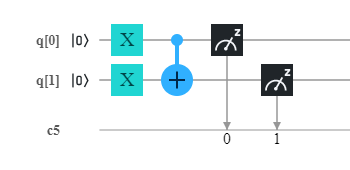
\includegraphics[width=.9\textwidth]{./img/IBMregisters.png}
\end{center}
\end{subfigure}%
\begin{subfigure}{.5\textwidth}
\leavevmode
\begin{center}
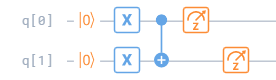
\includegraphics[width=.9\textwidth]{./img/QIregisters.png}
\end{center}
\end{subfigure}
\caption{circuit visualisatie bij IBM(l) en QI(r). Bij beide engines is het resultaaat 100\% 01.  Het 'LSB' is dus boven:$\ket{TC}$}
\label{fig:IBMQIcircuits}
\end{figure}

\iffalse%lukt even niet
\marginpar{\begin{tikzpicture}[>=stealth]
\matrix (A) [matrix of nodes,row sep=3mm,column sep=3mm,nodes in empty cells]
{
$\ket{00}$   & & & $\ket{00}$\\
$\ket{01}$   & & & $\ket{01}$\\
$\ket{10}$   & & & $\ket{10}$\\
$\ket{11}$   & & & $\ket{11}$\\
};
\begin{scope}[thick,red,<->]
\draw (A-1-1)--(A-1-4);
\draw (A-2-1)--(A-2-4);
\draw (A-3-1)--(A-4-4);
\draw (A-4-1)--(A-3-4);
\end{scope}
\end{tikzpicture}
}
\fi
De matrixvorm van de CNOT is 4x4, we moeten inmmers twee bits bijhouden.
$CNOT = \smqty(1&0&0&0\\0&1&0&0\\0&0&0&1\\0&0&1&0)$

We schrijven het nog twee keer uit:

$
CNOT\ket{10}=CNOT
\mqty(\mqty(0\\1)\otimes\mqty(1\\0))=
\mqty(1&0&0&0\\0&1&0&0\\0&0&0&1\\0&0&1&0)\mqty(0\\0\\1\\0)=
\mqty(0\\0\\0\\1)=\mqty(0\\1)\otimes\mqty(0\\1)=
\ket{11}
$

$
CNOT\ket{11}=CNOT
\mqty(\mqty(0\\1)\otimes\mqty(0\\1))=
\mqty(1&0&0&0\\0&1&0&0\\0&0&0&1\\0&0&1&0)\mqty(0\\0\\0\\1)=
\mqty(0\\0\\1\\0)=
\mqty(0\\1)\otimes\mqty(1\\0)=
\ket{10}$

\end{document}